\documentclass[letterpaper]{article} % DO NOT CHANGE THIS
\usepackage[submission]{aaai2026}  % DO NOT CHANGE THIS
\usepackage{times}  % DO NOT CHANGE THIS
\usepackage{helvet}  % DO NOT CHANGE THIS
\usepackage{courier}  % DO NOT CHANGE THIS
\usepackage[hyphens]{url}  % DO NOT CHANGE THIS
\usepackage{graphicx} % DO NOT CHANGE THIS
\urlstyle{rm} % DO NOT CHANGE THIS
\def\UrlFont{\rm}  % DO NOT CHANGE THIS
\usepackage{natbib}  % DO NOT CHANGE THIS AND DO NOT ADD ANY OPTIONS TO IT
\usepackage{caption} % DO NOT CHANGE THIS AND DO NOT ADD ANY OPTIONS TO IT
\usepackage{amsmath}
\usepackage{amssymb}
\usepackage{array}
\usepackage{booktabs}
\frenchspacing  % DO NOT CHANGE THIS
\setlength{\pdfpagewidth}{8.5in} % DO NOT CHANGE THIS
\setlength{\pdfpageheight}{11in} % DO NOT CHANGE THIS
%
% These are recommended to typeset algorithms but not required. See the subsubsection on algorithms. Remove them if you don't have algorithms in your paper.
\usepackage{algorithm}
\usepackage{algorithmic}

%
% These are are recommended to typeset listings but not required. See the subsubsection on listing. Remove this block if you don't have listings in your paper.
\usepackage{newfloat}
\usepackage{listings}
\DeclareCaptionStyle{ruled}{labelfont=normalfont,labelsep=colon,strut=off} % DO NOT CHANGE THIS
\lstset{%
	basicstyle={\footnotesize\ttfamily},% footnotesize acceptable for monospace
	numbers=left,numberstyle=\footnotesize,xleftmargin=2em,% show line numbers, remove this entire line if you don't want the numbers.
	aboveskip=0pt,belowskip=0pt,%
	showstringspaces=false,tabsize=2,breaklines=true}
\floatstyle{ruled}
\newfloat{listing}{tb}{lst}{}
\floatname{listing}{Listing}
%
% Keep the \pdfinfo as shown here. There's no need
% for you to add the /Title and /Author tags.
\pdfinfo{
/TemplateVersion (2026.1)
}

\setcounter{secnumdepth}{0} %May be changed to 1 or 2 if section numbers are desired.

% Title
\title{Interpretable Machine Learning for Predicting Adverse Drug Interactions in Singapore}
\author{
    % Authors - Replace with actual names
    An Xiao\textsuperscript{\rm 1},
    Liu Lexi\textsuperscript{\rm 2},
    Zhou Zirun\textsuperscript{\rm 3}
}
\affiliations{
    % Affiliations
    \textsuperscript{\rm 1}School of Computing, National University of Singapore\\
    student1@nus.edu.sg, student2@nus.edu.sg, student3@nus.edu.sg
}

\begin{document}

\maketitle

\begin{abstract}
The rapid advancement of healthcare systems and increased life expectancy have led to a growing prevalence of polypharmacy, particularly among elderly patients in Singapore. This paper proposes an interpretable machine learning application to predict the risk of adverse drug interactions, providing transparent explanations to support clinical decision-making tailored to the Singapore context.
\end{abstract}

\section{Introduction}

The rapid advancement of healthcare systems and increased life expectancy have led to a growing prevalence of polypharmacy, where patients—particularly elderly individuals—are prescribed multiple medications simultaneously. While such multi-drug therapies are often necessary for managing chronic conditions, they significantly increase the risk of drug-drug interactions (DDIs). Statistics show that DDIs may greatly contribute to a worsening patient condition through adverse side effects.\cite{Chan2016:chan}, and the risk of DDIs is underperceived by the medical industry.\cite{polypharmacy}

DDI is especially critical in Singapore.\cite{Ho2023} Given that there is a vacuum in reliable formal methods among Singaporean doctors to avoid drug interactions, we propose to leverage machine learning algorithms to provide explainable advice to Singaporean doctors on possible drug interactions for every prescription. We first show that drug interaction is an important issue that can be properly addressed through machine learning algorithm under Singaporean context. We will then expound on the further details in our choice of the machine learning algorithm and its training process. Last but not the least, we will demonstrate the result of our prototypical machine learning application and how it benefits Singapore's medical industry through providing explainable advice on potential drug interactions in prescriptions.


\section{Motivation}

\subsection{Drug interactions as a severe issue in Singapore}

DDI has been recognised as a significant contributor to the degeneration of patient health \cite{polypharmacy,Chan2016:chan}. The complexity of managing multiple medications increases the likelihood of unintended interactions, making it crucial for healthcare providers to have effective tools for predicting and preventing DDIs.

Singapore presents a particularly important context for addressing this problem. First, the country's demographic structure is shifting toward an ageing society, with a high proportion of elderly individuals requiring long-term medication.\cite{singstat_population_2025} Figure 1 shows our rough estimate of the elderly population in Singapore in 2025 based on the age distribution of the population and the stratified death rate of different age groups\cite{singstat_death_rate_2025} in Singapore in 2025. With aging population, the number of senior citizen is expected to proliferate in the upcoming decades, which indicates a sharp increase in the demand of polypharmacy due to the positive association between seniority of an individual to more complex medication needs.\cite{Ho2023,Wong2019} 

\begin{figure}[t]
    \centering
    \includegraphics[width=0.95\columnwidth]{./population.png}
    \caption{Predicted elderly Population(above 60) of Singapore in 2025.}
    \label{fig:population_pyramid}
\end{figure}

Second, Singapore exhibits a unique disease profile, with high rates of metabolic and cardiovascular conditions, which often necessitate multi-drug treatment plans.\cite{hop_health_concerns_2025} 

Third, the healthcare system in Singapore emphasises precision medicine and efficient clinical decision-making, creating a strong demand for tools that can assist healthcare professionals in evaluating complex prescription combinations.Even though there are drug interaction database and alogrithms available, the data are mostly collected from a more Western profile. The bias in the data collected may lead to potential underrepresentation of certain diseases that are more common among Singaporeans. The underrepresentation indicates that the current algorithms may not be the most appropriate under Singaporean context and there is a significant space for improvement for us.  

\subsection{Why machine learning algorithms}

Machine learning has been effective in detecting patterns of drug interactions as it can be categorised as a classification task.\cite{Gheorghita2025} When the number of drugs involved in a single prescription increase, we expect the number of possible pair of drugs that may produce interaction to increase exponentially($N =$ $n\choose2$, n is the number of drugs and N is the number of possible pairs), which eventually leads to human oversight. 

Even though there are available databases nowadays where doctors can use for reference. Machine learning alogrithm further enhances drug interaction detection as it is able to predict the reaction purely through the chemical structure of the drugs. This capability is relevant to Singapore context as most of the databses are constructed through European countries or the united states where some prescriptions more commonly utilised in Singapore may be unavailable because of different diesease profiles.

We can further leverage the strengths of interpretable ML models—such as their ability to provide human-understandable decision rules and feature contributions—to ensure that medical professionals can trust and effectively utilise the model's predictions. More details will be explored in the solution section.

\subsection{Ethical considerations}

While the previous sections mention the advantages of using machine learning algorithms to detect drug interactions, we also acknowledge the important ethical considerations as the healthcare industry typically involves high-stake responsibilities where many believe that human decisions must be involved. Drug prescription is no exception. 

First, any misjudgement by the algorithm must be held accountable. The machine learning algorithm can never make any independent judgement on its own without human oversight. The patient, who are unable to judge the accuracy of the predicted drug interaction result, should also not be exposed to the decision making process. Therefore, we envision the algorithm to be most ethically positioned as advisory to the doctors, with which the doctor gives the final decision on whether the drug interaction may actually happen and be held accountable for his own judgement as a medical professional.

\section{Method}

We first define the input and the output of our machine learning model. The input is a pair of drugs and the patient's condition, and the output contains the possibility predicted about whether the two drugs interact with each other.
We mathematically express our model as follows:

\begin{equation}
    \hat{y} = F(D_A, D_B)
\end{equation}

where $D_A, D_B \in \mathbb{R}^{d}$ are the molecular fingerprints of Drug A and Drug B with dimension $d$, respectively, and $c$ is the patient's condition vector. The function $F$ represents the machine learning model that takes these inputs and produces a prediction $\hat{y}$ indicating the probability of an interaction. In our experiment, we use random forest  as our machine learning models, which will be further explained in the next section.

Then with the output possibility $\hat{y}$, we can further apply a threshold to determine whether the drug pair is predicted to interact or not. For example, if $\hat{y} > 0.3$, we can classify the drug pair as interacting; otherwise, we classify it as non-interacting. After interacting pairs are identified, we can further provide an explanation of the interaction through the interpretable machine learning model, which will be discussed in the next section.

Additionally, with the predicted interaction, we can further predict the severity of the interaction of the drug pair. For example, we can classify the severity into three levels: mild, moderate, and severe based on the patient's condition and the predicted interaction. This can be achieved by training a separate model that takes the predicted interaction and patient's condition as input and outputs the severity level.

\subsection{Datasets and Data Structures}

\subsubsection{Data Source}
\ 
\newline
For drug interactions, we use the \textbf{BIOSNAP ChChMiner} dataset, which is derived from DrugBank and contains experimentally validated drug-drug interaction (DDI) pairs. Each entry in the raw dataset consists of two DrugBank IDs indicating that the pair of drugs is known to interact and should not be used together. After filtering out drug pairs for which molecular structures could not be retrieved, our dataset contains approximately 40,000 positive examples (interacting pairs). 

The BIOSNAP dataset only contains known positive interactions. Since no ground-truth negative pairs are provided, we construct negative examples by randomly sampling drug pairs that do not appear in the positive set. We follow the standard 1:1 positive-to-negative ratio. We acknowledge that this procedure relies on the assumption that pairs absent from DrugBank are treated as non-interacting, though some may represent undiscovered interactions. This is a well-recognised limitation of DDI benchmarks and is consistent with prior work in this area.

Considering paitent condition, we use \textbf{FDA FARES} dataset, which contain reports of patients having adverse reactions after taking certain combination of drugs with their personal information about age, gender and etc.with the patients' consent.

\subsubsection{Molecular Feature Representation}
\ 
\newline
Each drug is represented as a 166-dimensional binary fingerprint generated using the MACCS Keys (Molecular ACCess System) scheme via RDKit. MACCS Keys encode the presence or absence of 166 predefined chemical substructures, such as the presence of a benzene ring (Key 120), a carboxyl group (Key 148), or a nitrogen-containing heterocycle (Key 80). Each bit is either 1 (substructure present) or 0 (absent).

During data preprocessing, we removed MACCS bits with zero across all drugs in the dataset, which also means the bits representing chemicals that are universally universally absent. These chemical strucutres are not conventionally used in drugs and their removal reduces noise in the input representation. After this filtering step, the effective fingerprint dimensionality is reduced from 166 to 162 bits per drug, resulting in a final feature vector of 324 dimensions per drug pair.

We chose MACCS Keys over the more commonly used Morgan fingerprints mainly because each MACCS bit corresponds to a named, chemically interpretable substructure, which directly supports our interpretability analysis.


\subsection{Input construction}

\subsubsection{Drug Interaction Pairs}
\
\newline
For the input, we represent each drug using its molecular fingerprint represented by MACCS keys. MACCS keys converts chemical structures into a binary vector of 166 dimensions based on the presence or absence of specific chemical substructures.\cite{rdkit} It is also widely adpoted in pharmaceutical research as a form of data representation of drugs\cite{xie2020improvement,durant2002reoptimization} The model learns to predict the interaction label based on the combined features of the two drugs.
For instance, the 120 th dimension of the input vector indicates the presence of a benzene ring.\cite{rdkit} 

However, to study the pair of drugs as the input, we need to combine their molecular fingerprints into a single vector. In other words, 
\begin{center}$x = g(D_A, D_B)$
\end{center}
where $g$ is the function that combines the two drug fingerprints into a single input vector.

The function $g$ should satisfy two properties.

First, it should be \textbf{symmetric}, or $g(D_A, D_B) = g(D_B, D_A)$

Second, the function should \textbf{preserve the interpretability of the features}, allowing us to understand which chemical substructures contribute to the predicted interaction.
There are several possible ways to combine the two drug fingerprints, such as concatenation, element-wise multiplication, or addition. We choose to use addition for its simplicity and interpretability. With element wise addition, the input vector for a drug pair is represented as:

\begin{equation}
    x_i = \begin{cases}
        0 & \text{if neither drug has the substructure} \\
        1 & \text{if exactly one drug has the substructure} \\
        2 & \text{if both drugs have the substructure} 
        \end{cases}
\end{equation}

where $x_i$ is the $i$-th dimension of the input vector, corresponding to the $i$-th MACCS key. 



\subsubsection{Patient Condition}
\
\newline
A simple binary vector will be used to represent the presence or absence of certain conditions that are relevant to drug interactions. This allows the model to consider how patient-specific factors may influence the likelihood and severity of drug interactions.

\subsection{Algorithm and models}
We decided to leverage random forest as the major model for prediction and explanation. Random forest is a powerful ensemble learning method that combines multiple decision trees to improve predictive performance and control overfitting. It is particularly well-suited for our task due to its ability to handle high-dimensional, sparse input data (like molecular fingerprints) and its inherent interpretability through feature importance measures and decision paths.

\subsubsection{Logistic Regression}
\ 
\newline
Logistic Regression serves as our linear baseline. It computes a weighted sum of all 324 input features and passes the result through a sigmoid function to produce an interaction probability:

\begin{equation}
    \hat{y} = \sigma(\mathbf{w}^T \mathbf{x} + b)
\end{equation}

Despite its simplicity, logistic regression provides a meaningful lower bound on performance and highlights the limitations of linear decision boundaries in this task.

\subsubsection{MLP}
\ 
\newline
Our Multi-Layer Perceptron consists of three fully-connected hidden layers with ReLU activations and dropout regularisation:

\begin{center}
    $324 \rightarrow 256 \rightarrow 128 \rightarrow 64 \rightarrow 1$
\end{center}
Dropout with probability 0.3 is applied after each of the first two hidden layers to reduce overfitting. The output layer uses a sigmoid activation to produce an interaction probability. The model is trained with the Adam optimiser (learning rate $10^{-3}$) and binary cross-entropy loss for 50 epochs, with the best checkpoint selected based on validation AUC-ROC.

Compared to Random Forest, the MLP learns a more sophisticated combination of possible chemical interactions between different drug pairs. Given the nature of the data encoding, where each index refers to the presence of certain chemical strucutres in the drug. We can express a simplified example as the following.

\begin{figure}[h!]
    \centering
    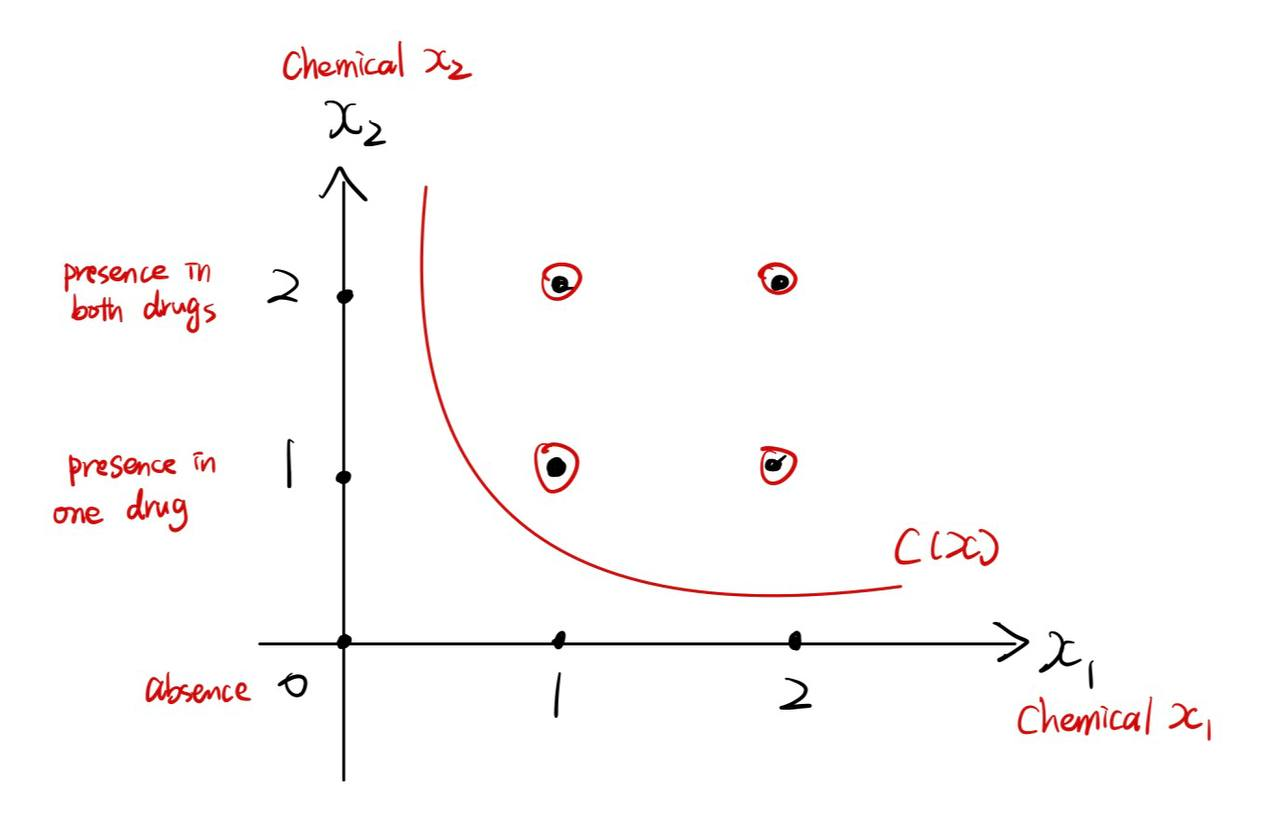
\includegraphics[width=0.95\columnwidth]{./MLP.png}
    \caption{A simple example of learning drug interactions with only two types of chemicals involved.}
    \label{fig:MLP}
\end{figure}

From the figure above, we assume that the true concept $c(x) = 1,  x_1 \geq 1 \text{ and } x_2 \geq 1$, which means that the presence of both chemical $x_1$ and $x_2$ in the target drug pair will lead to an adverse interaction. We can then utilise the universal approximation theorem of neural networks to claim that this true function is recoverable thorugh MLP. 

The particular relationship presented in the figure cannot be captured through naive logistic regression without any feature transformation since the size of input instance space $|X| = 8$ while $VC(H) = 3 < 8$ when the hypothesis space consists of all linear combinations of $x_1$ and $x_2$. On the other hand, MLP leverages on the universal approximation theroem which allows any polynomial continuous functions to be accurately approximated with sufficient number of neurons.

However, a major limitation of MLP alogrithm is its difficulty in prvoding an interpretable explanation to the doctor when advising possible drug interactions. First, the MLP learns the true function through universal approximation theorem which makes it impossible to recover the true function that MLP is approximating towards. Second, given that chemical reactions take place indepedently, MLP conflates all chemical reactions in one single hypothesis which makes it difficult to retreive the separate reactions that may take place between two drugs.

\subsubsection{Random Forest}
\
\newline
\paragraph{Algorithm Overview.}
Random Forest, introduced by \citet{Breiman2001}, is a non-parametric ensemble method that combines the predictions of $T$ independently trained decision trees to reduce variance while retaining the low bias of individual trees. Each tree $\mathcal{T}_t$ ($t = 1, \ldots, T$) is trained on a bootstrap resample $\mathcal{D}_t \sim \text{Bootstrap}(\mathcal{D})$ drawn \emph{with replacement} from the full training set $\mathcal{D} = \{(\mathbf{x}_i, y_i)\}_{i=1}^{n}$, where $\mathbf{x}_i \in \mathbb{R}^{p}$ and $y_i \in \{0, 1\}$. This procedure, known as \emph{bagging} \cite{Breiman1996}, ensures that each tree sees a different perturbation of the data, thereby decorrelating the ensemble members.
 
\paragraph{Tree Construction via CART.}
Every tree is grown using the Classification and Regression Tree (CART) algorithm \cite{Breiman1984}. At each internal node $v$ with sample set $S_v$, CART selects the feature index $j^*$ and threshold $\tau^*$ that minimise the weighted Gini impurity of the resulting split:
\begin{equation}
    (j^*, \tau^*) = \arg\min_{j \in \mathcal{M}_v,\; \tau}
    \frac{|S_L|}{|S_v|}\, G(S_L) + \frac{|S_R|}{|S_v|}\, G(S_R),
    \label{eq:cart_split}
\end{equation}
where $S_L = \{\mathbf{x} \in S_v : x_j \leq \tau\}$, $S_R = S_v \setminus S_L$, and the Gini impurity of a node $S$ is
\begin{equation}
    G(S) = 1 - \sum_{k \in \{0,1\}} \hat{p}_k^2, \quad
    \hat{p}_k = \frac{|\{\mathbf{x} \in S : y = k\}|}{|S|}.
    \label{eq:gini}
\end{equation}

\paragraph{Ensemble Prediction.}
Given $T$ fitted trees, the predicted interaction probability for a drug pair $\mathbf{x}$ is the average of the per-tree leaf class probabilities:
\begin{equation}
    \hat{y} = F(\mathbf{x}) = \frac{1}{T} \sum_{t=1}^{T} \hat{p}_t(\mathbf{x}),
    \label{eq:rf_pred}
\end{equation}
where $\hat{p}_t(\mathbf{x})$ is the fraction of positive training samples in the leaf node of tree $\mathcal{T}_t$ that $\mathbf{x}$ falls into. A binary prediction is obtained by thresholding $\hat{y}$ against a chosen operating point $\delta$:

 In our experiments, we train a forest of $T = 100$ trees using the \texttt{sklearn} defaults: $m = \lfloor\sqrt{p}\rfloor$, unlimited tree depth, and minimum samples per leaf of 1.

\paragraph{Applicability to This Task.}
Several properties of the DDI task make Random Forest a principled model choice.
 
\textit{(i) Ordinal feature space.} Our combined drug-pair fingerprint $\mathbf{x} \in \{0, 1, 2\}^{p}$ arises from element-wise addition of two MACCS binary vectors. Each coordinate takes one of three ordinal integer values, and CART splits of the form $x_j \leq \tau$ partition this space without requiring any normalisation or distributional assumption, which is particularly important for chemical fingerprint data \cite{Svetnik2003}.
 
\textit{(ii) Accurate capturing of potential drug interactions through decision boundaries.} CART naturally encodes conjunctive rules: a single path from root to leaf can represent conditions such as ``$x_j = 2$ (both drugs must share the same substance) \emph{and} $x_k, x_r \geq 1$ (Both drugs together contain chemeicals represented by index $k$ or $r$ that may interact with each other).'' Moreover, given that drug interaction mechanisms can operate through largely independent biological pathways, random forest's ensemble strategy — which exploits decorrelated, parallel trees — is theoretically well-suited to this domain. In fact, Random forests have been shown to be effective for DDI prediction on molecular fingerprints in several prior studies\cite{Gottlieb2012,Vilar2012,Ryu2018}.
 
\subsubsection{Interpretability via Tree-Ranked Decision Path Output}
\
\newline
A global feature importance metric such as Mean Decrease in Impurity
(MDI) describes average behaviour across the entire training set.
Our earlier PDP formulation aggregated isolated split conditions across
all positive-voting trees, producing a ranked list of individual
conditions.  Here we adopt a structurally richer strategy: we
\emph{rank the trees themselves} and, for each top-ranked tree, output
its \emph{complete} root-to-leaf decision path.  A full path is a
conjunction of conditions — a single, coherent if-then rule — and is
therefore directly interpretable by a clinician without further
aggregation.
 
\paragraph{Decision Path of a Single Tree.}
For a test sample $\mathbf{x}$ and tree $\mathcal{T}_t$, define the
\emph{decision path} as the ordered sequence of split conditions
encountered from the root to the reached leaf:
\begin{equation}
    \Pi_t(\mathbf{x}) =
    \bigl(c_1^{(t)},\; c_2^{(t)},\; \ldots,\; c_{d_t}^{(t)}\bigr),
    \label{eq:path}
\end{equation}
where each condition is the triple
$c_l^{(t)} = \bigl(j_l^{(t)},\; \tau_l^{(t)},\; \delta_l^{(t)}\bigr)$,
with $j_l^{(t)}$ the MACCS key index, $\tau_l^{(t)} \in \{0.5, 1.5\}$
the split threshold, $\delta_l^{(t)} \in \{\leq, >\}$ the branch
direction taken by $\mathbf{x}$, and $d_t$ the path depth.
The path $\Pi_t(\mathbf{x})$ encodes the following conjunction rule:
\begin{equation}
    \bigwedge_{l=1}^{d_t}
    \Bigl(x_{j_l^{(t)}} \;\delta_l^{(t)}\; \tau_l^{(t)}\Bigr)
    \;\Longrightarrow\; \tilde{y} = 1.
    \label{eq:conjunction}
\end{equation}
Because $\tau_l^{(t)} \in \{0.5, 1.5\}$ and $x_j \in \{0,1,2\}$,
every condition in \eqref{eq:conjunction} maps to one of two
semantically precise chemical statements per MACCS key $j$:
\begin{align}
    x_j > 0.5 &\;\Longleftrightarrow\;
        \text{at least one drug in the pair has substructure } j,
        \label{eq:sem_one}\\
    x_j > 1.5 &\;\Longleftrightarrow\;
        \text{both drugs in the pair share substructure } j,
        \label{eq:sem_both}\\
    x_j \leq 0.5 &\;\Longleftrightarrow\;
        \text{neither drug in the pair has substructure } j.
        \label{eq:sem_none}
\end{align}
 
\paragraph{Restricting to Positive-Voting Trees.}
Only trees that individually voted for an interaction carry explanatory
relevance for the positive prediction.  Define the set of
\emph{positive-voting trees} as
\begin{equation}
    \mathcal{T}^{+}(\mathbf{x}) =
    \bigl\{t \in \{1,\ldots,T\} : \hat{p}_t(\mathbf{x}) > 0.5\bigr\},
    \label{eq:pos_trees}
\end{equation}
where $\hat{p}_t(\mathbf{x})$ is the fraction of positive training
samples in the leaf of tree $\mathcal{T}_t$ reached by $\mathbf{x}$.
The ensemble predicts a positive interaction when
$|\mathcal{T}^{+}(\mathbf{x})| > T/2$, so $\mathcal{T}^{+}(\mathbf{x})$
is guaranteed to be non-empty whenever $\tilde{y} = 1$.
 
\paragraph{Ranking Trees by Leaf Confidence.}
Not all positive-voting trees are equally informative as explanations.
A tree whose reached leaf contains 95\% positive training samples made
a highly decisive vote; a tree at 51\% barely cleared the threshold and
its path reflects a weakly discriminative rule.  We rank trees by their
\emph{leaf confidence}, defined as
\begin{equation}
    \psi(t, \mathbf{x}) = \hat{p}_t(\mathbf{x}),
    \label{eq:tree_score}
\end{equation}
and sort $\mathcal{T}^{+}(\mathbf{x})$ in descending order of
$\psi(t, \mathbf{x})$.  The top-$K$ trees in this ranking,
\begin{equation}
    \mathcal{T}^{*}(\mathbf{x}) =
    \operatorname*{arg\,top\text{-}K}_{t\;\in\;\mathcal{T}^{+}(\mathbf{x})}
    \;\psi(t, \mathbf{x}),
    \label{eq:top_k}
\end{equation}
are selected as the explanation representatives.
A natural default is $K = 1$ (the single most confident positive-voting
tree), which produces a minimal, easily communicated rule.
Setting $K > 1$ surfaces alternative rule sets that independently
support the prediction, giving the clinician a sense of how
structurally diverse the forest's reasoning is.
 
\paragraph{Full-Path Output.}
For each tree $t \in \mathcal{T}^{*}(\mathbf{x})$, ranked by confidence,
we output the complete decision path $\Pi_t(\mathbf{x})$ as an ordered
list of $d_t$ human-readable conditions.  For example, the top-ranked
tree's explanation might read:
\begin{quote}
\emph{Tree rank 1 (leaf confidence $= 0.94$):}\\
\emph{[Node 1]\; Key 120 $> 0.5$\;
$\Rightarrow$ at least one drug has a benzene ring.}\\
\emph{[Node 2]\; Key 148 $> 1.5$\;
$\Rightarrow$ both drugs carry a carboxyl group.}\\
\emph{$\Rightarrow$ \textbf{Predicted: Interaction.}}
\end{quote}

This format is structurally analogous to a clinical decision rule, a format already familiar to medical professionals \cite{Rudin2019}. Each node corresponds to a testable chemical property; taken together, the conjunction rule constitutes a complete, falsifiable hypothesisabout why the interaction is predicted.
 
\paragraph{Relationship to SHAP.}
SHAP TreeExplainer \cite{Lundberg2020} produces a continuous attribution score $\phi_j$ per feature, computed as the average marginal
contribution of feature $j$ across all feature orderings.The tree-ranked path approach is complementary: it provides the exact internal conjunction rule fired by the most confident tree, without any averaging or approximation. The two methods can be cross-validated by checking whether the top-$K$ MACCS keys appearing in $\Pi_{t^*}(\mathbf{x})$ (the most-confident tree's path) also carry high absolute SHAP values $|\phi_j|$.  Strong agreement indicates that the explanation is robust across both local-faithful and marginal-contribution perspectives.
 


\section{Expreiment Process}
\subsubsection{Dataset splits}
\ 
\newline
The final dataset is split into training, validation, and test sets at an 80/10/10 ratio, with stratification to preserve the class balance across all splits.
\subsection{MLP}
\subsection{Random Forest}
\section{Results}
\bibliography{CS3264_Final_Report}
\section{appendix}

\subsection*{Appendix A: Notation}
 
Table~\ref{tab:notation} summarises all mathematical symbols used in
the Random Forest and Tree-Ranked Decision Path (TRDP) sections.
 
\begin{table}[h]
\centering
\caption{Mathematical notation for the Random Forest and TRDP sections.}
\label{tab:notation}
\renewcommand{\arraystretch}{1.25}
\begin{tabular}{>{\(}c<{\)} p{5.6cm}}
\toprule
\textbf{Symbol} & \textbf{Description} \\
\midrule
 
%% ----- Dataset -----
\multicolumn{2}{l}{\textit{Dataset}} \\[2pt]
\mathcal{D}
    & Full labelled training set $\{(\mathbf{x}_i, y_i)\}_{i=1}^{n}$ \\
n
    & Number of training samples \\
p
    & Feature dimensionality; $p = 324$ after MACCS preprocessing \\
\mathbf{x}_i
    & Feature vector of training sample $i$,
      $\mathbf{x}_i \in \mathbb{R}^{p}$ \\
y_i
    & Binary interaction label, $y_i \in \{0,1\}$ \\
\mathbf{x}
    & Query drug-pair feature vector (test sample),
      $\mathbf{x} \in \{0,1,2\}^{p}$ \\
x_j
    & $j$-th coordinate of $\mathbf{x}$, corresponding to MACCS key $j$;
      $x_j \in \{0,1,2\}$ \\
k
    & Class index, $k \in \{0,1\}$
      ($0$ = non-interacting, $1$ = interacting) \\
 
\midrule
%% ----- Ensemble -----
\multicolumn{2}{l}{\textit{Ensemble (Forest Level)}} \\[2pt]
T
    & Total number of trees in the forest \\
t
    & Tree index, $t \in \{1, \ldots, T\}$ \\
\mathcal{T}_t
    & The $t$-th decision tree \\
\mathcal{F}
    & Fitted forest $\{\mathcal{T}_t\}_{t=1}^{T}$ \\
\mathcal{D}_t
    & Bootstrap resample used to train tree $t$,
      drawn with replacement from $\mathcal{D}$ \\
F(\mathbf{x})
    & Ensemble prediction function;
      outputs the predicted interaction probability \\
\hat{y}
    & Predicted interaction probability,
      $\hat{y} = F(\mathbf{x}) \in [0,1]$ \\
\tilde{y}
    & Binary interaction prediction,
      $\tilde{y} = \mathbf{1}[\hat{y} > \theta]$ \\
\theta
    & Classification threshold applied to $\hat{y}$ to produce
      $\tilde{y}$ \\
\hat{p}_t(\mathbf{x})
    & Fraction of positive training samples in the leaf of tree
      $\mathcal{T}_t$ reached by $\mathbf{x}$;
      serves as the per-tree class probability and confidence score \\
\rho
    & Average pairwise correlation between trees in the ensemble \\
\sigma^2
    & Per-tree prediction variance \\
\mathrm{Var}[F]
    & Variance of the ensemble predictor $F$ \\
 
\midrule
%% ----- CART node level -----
\multicolumn{2}{l}{\textit{Node Level (CART Tree Construction)}} \\[2pt]
v
    & An internal node in a decision tree \\
S_v
    & Set of training samples routed to node $v$ \\
S_L,\;S_R
    & Left and right child sample sets produced by a split at $v$ \\
j
    & Candidate split feature index, $j \in \{1,\ldots,p\}$ \\
j^*
    & Optimal split feature index selected by CART at a given node \\
\tau
    & Candidate split threshold \\
\tau^*
    & Optimal split threshold selected by CART at a given node \\
\mathcal{M}_v
    & Random feature subset considered at node $v$,
      $\mathcal{M}_v \subseteq \{1,\ldots,p\}$ \\
m
    & Size of the random feature subset,
      $m = \lfloor\sqrt{p}\rfloor$ \\
G(S)
    & Gini impurity of a sample set $S$;
      $G(S) = 1 - \sum_{k}\hat{p}_k^{\,2}$ \\
\hat{p}_k
    & Fraction of class-$k$ samples in a node:
      $|\{\mathbf{x}{\in}S : y{=}k\}|\,/\,|S|$ \\
\hat{p}
    & Shorthand for $\hat{p}_1$, the fraction of positive samples
      in a node (binary case) \\
d_{\max}
    & Maximum depth across all trees in the forest \\
d_{\max}^{\mathrm{report}}
    & Maximum number of path nodes reported to the clinician
      (post-hoc display cap; does not affect model training) \\
 
\midrule
%% ----- TRDP interpretability -----
\multicolumn{2}{l}{\textit{TRDP Analysis (Interpretability)}} \\[2pt]
\Pi_t(\mathbf{x})
    & Ordered sequence of split conditions along the root-to-leaf
      path of tree $\mathcal{T}_t$ for query $\mathbf{x}$ \\
c_l^{(t)}
    & The $l$-th split condition in the path of tree $t$;
      a triple $(j_l^{(t)}, \tau_l^{(t)}, \delta_l^{(t)})$ \\
c
    & A generic condition triple $(j,\tau,\delta)$ when the
      tree index is implicit \\
j_l^{(t)}
    & MACCS key index of the split at depth $l$ in tree $t$ \\
\tau_l^{(t)}
    & Split threshold at depth $l$ in tree $t$;
      $\tau_l^{(t)} \in \{0.5,\,1.5\}$ for ordinal features \\
\delta_l^{(t)}
    & Branch direction taken by $\mathbf{x}$ at depth $l$ in tree $t$;
      $\delta_l^{(t)} \in \{\leq,\,>\}$ \\
d_t
    & Depth of the path in tree $t$
      (number of internal nodes traversed) \\
l
    & Depth index along a root-to-leaf path,
      $l \in \{1,\ldots,d_t\}$ \\
\mathcal{T}^{+}(\mathbf{x})
    & Set of positive-voting trees for sample $\mathbf{x}$:
      $\{t : \hat{p}_t(\mathbf{x}) > 0.5\}$ \\
\psi(t,\mathbf{x})
    & Tree ranking score (leaf confidence) for tree $t$ on sample
      $\mathbf{x}$; defined as $\hat{p}_t(\mathbf{x})$ \\
\mathcal{T}^{*}(\mathbf{x})
    & Top-$K$ trees from $\mathcal{T}^{+}(\mathbf{x})$ ranked by
      $\psi(t,\mathbf{x})$ in descending order \\
K
    & Number of top-ranked trees whose full paths are reported
      as explanations \\
\phi_j
    & SHAP attribution score for feature $j$
      (used for cross-validation against TRDP output) \\
\bottomrule
\end{tabular}
\end{table}

\end{document}
